\documentclass[a4paper, 10pt, notitlepage]{article}

\usepackage{moreverb} %para importar codigo

\usepackage{caratula} %paquete personal para la caratula del DC

\usepackage[spanish,activeacute]{babel}
\usepackage{babel} %paquete de idioma

\usepackage[latin1]{inputenc}

\usepackage{color}

\usepackage{fancyhdr} %linea sup con comentarios

%\usepackage{listings}

\usepackage{lscape} %para hoja apaisada

\usepackage{framed} %para crear cajas de texto

\usepackage{lastpage} %ultima pagina

\addtolength{\topmargin}{-50pt} 
\addtolength{\textwidth}{105pt}
\addtolength{\textheight}{120pt}
\addtolength{\oddsidemargin}{-50pt}

\newcommand{\cuat}{1er cuatrimestre de 2007}
\newcommand{\au}{``�rbol �nico''}
\newcommand{\da}{``Dos �rboles''}
\newcommand{\ada}{``�rbol de �rboles''}
\newcommand{\aac}{``�rbol con ambas coordenadas''}

%%% Encabezado y pie de p'agina
\pagestyle{fancy}
\fancyhead[LO]{Algoritmos y Estructura de Datos III}
\fancyhead[C]{}
\fancyhead[RO]{P\'agina \thepage\ de \pageref{LastPage}}
\renewcommand{\headrulewidth}{0.4pt}
\fancyfoot{}

\newcommand{\rbt}{\textit{ �rbol {\color{red}\textbf{Rojo}} y \textbf{Negro}} }
\newcommand{\adi}{\textit{ �rbol de \textbf{Intervalos} }}

\begin{document}
\titulo{}
\subtitulo{Trabajo Pr\'actico - $N^o$ 2}
\fecha{Algoritmos y Estructura de Datos III}
\materia{1er cuatrimestre 2007}
\submateria{}
\integrante{Garc\'ia, Ana Daniela}{530/05}{danita719@yahoo.com.ar}
\integrante{Joaquin Miguez}{120/04}{jmiguez@dc.uba.ar}
\integrante{Fernando Bugni}{611/05}{fernando.bugni@gmail.com}
\integrante{Engler, Christian Alejandro}{314/05}{caeycae@gmail.com}
%\logoimagefile{animaniacs.jpg}

%caratula
%\maketitle{}

%enunciado
%%%%%%%%%%%%%%%%%%%%%%%%%%%%%%%%%%%%%%%%%%%%%%%%%%%%%%%%%%%%%%%%%%%%%%%%%%%%%%%%%%%%%%%%%%%%%
\section{Introducci\'on}
%%%%%%%%%%%%%%%%%%%%%%%%%%%%%%%%%%%%%%%%%%%%%%%%%%%%%%%%%%%%%%%%%%%%%%%%%%%%%%%%%%%%%%%%%%%%
\subsection{Enunciado}

\begin{framed}	

\begin{center}

\hspace{1cm}

\LARGE
UBA - FCEyN - Departamento de Computaci�n\\
\large
ALGORITMOS Y ESTRUCTURAS DE DATOS III\\
Trabajo Pr�ctico $N^o$ 1\\
Primera entrega: 7-5-2007, hasta las 19:30 horas\\
Segunda entrega: 28-5-2007, hasta las 19:30 horas\\
\small
Ver informaci�n general sobre los Trabajos Pr�cticos en la p�gina de la materia en Internet.
\end{center}

\hspace{1cm}

Ver informaci�n general sobre los Trabajos Pr�cticos en la p�gina de la materia en Internet.
El Booble art es un programa que muestra el mapa de Buenos Aires y sus atracciones tur�sticas. A medida que vamos recorriendo el mapa en la pantalla, podemos hacer un click en un punto y nos muestra varias fotos que corresponden a lugares que est�n cerca del punto que marcamos.

Nuestro objetivo es realizar un algoritmo que, dado un punto en el plano (la pantalla), decida cu�les son las fotos a mostrar.
Para esto, vamos a considerar los siguientes criterios:

\begin{itemize}
\item Cada foto tiene una posici�n en el plano dada por sus coordenadas.
\item La pantalla tiene un tama�o fijo de $s * t$
\item Al clickear en un punto del plano, las fotos que deben mostrarse son TODAS aquellas fotos que contienen a ese punto (es decir, el punto est� dentro del �rea dado por las coordenadas de la foto).
\item Las fotos pueden tener diferentes tama�os, intersecarse, estar contenidas una dentro de otra, etc.
\item Por supuesto, al listar las fotos a mostrar, pueden haber fotos que se intersecan, etc. Esto no nos preocupa, s�lo queremos conocer la lista de fotos a mostrarse en otra pantalla, donde otro programa (que se har� en Algoritmos 4) acomodar� estas fotos 
\end{itemize}

Vamos a realizar un preprocesamiento del conjunto de fotos para luego, cada vez que se realiza un click, podamos decidir qu� fotos deben mostrarse en forma eficiente.

\begin{enumerate}
\item (a) Dada un conjunto de fotos, construir un $arbol de intervalos$ usando \textbf{�rboles red black} (ser� explicado en clase) con las operaci�n $Insertar$.\vskip0.1cm
(b) Indicar el orden de las operaci�n $insertar$ No es obligatorio que figure en el informe la justificaci�n del orden de $insertar$ pero se preguntar� sobre esto durante el coloquio.\vskip0.1cm
(c) Calcular la complejidad \textsc{TEMPORAL Y ESPACIAL} de construir el �rbol de intervalos.\vskip0.1cm
(d) Dise�ar un algoritmo que, dado un punto en el plano, decida el conjunto de fotos a mostrar. Para esto, implementar la operaci�n $buscarInterseccion$.\vskip0.1cm
(e) Calcular la complejidad \textsc{TEMPORAL Y ESPACIAL} de realizar una consulta (llamamos ``consulta'' a clickear sobre un punto del plano).\vskip0.1cm
(f) Analizar el algoritmo midiendo el tiempo de ejecuci�n tanto para el armado del �rbol como para consultas. Es decir, para diferentes conjuntos de fotos (instancias), realizar varias consultas.\vskip0.1cm
\item Ahora, pensemos la siguiente variante. Cada tanto, el programa Booble art se actualiza y adiciona nuevas fotos a su mapa. Explicar c�mo cambia el algoritmo anterior, sus funciones, etc. Calcular la complejidad de la funci�n $insertar$ para este caso.
\end{enumerate}

Entrada \verb|Tp2Ej1.in| Este archivo contiene varias instancias de entrada. La primera l�nea contiene el n�mero de instancias. Cada instancia es definida de la siguiente manera. La primera l�nea contiene el n�mero de fotos $n$, las siguientes n l�neas contiene las coordenadas de las fotos: $x0$ $x1$ $y0$ $y1$, donde $x0 \leq x1$ y $y0 \leq  y1$.

\verb|Tp2Ej1d.in| Este archivo contiene consultas para hacer sobre todas las instancias del archivo anterior. La primera l�nea contiene la cantidad de consultas ($k$) y las siguientes $k$ l�neas contienen las coordenadas del punto del plano de la forma $x$ $y$.

NOTA: NO ES OBLIGATORIO QUE LA ENTRADA SE INGRESE POR LINEA DE COMANDOS, PERO EL QUE QUIERE PUEDE HACERLO DE AMBAS MANERAS.

Salida \verb|Tp2Ej4.out| Por cada instancia, cada l�nea contiene una foto que se debe mostrar identificada por sus cuatro coordenadas. La salida de cada instancias est� separada por un 0. 

Bibliograf�a: 

Fotocopiadora: ``Introduction to Algorithms'', Thomas H. Cormen, Charles E. Leiserson, Ronald L. Rivest, and Clifford Stein. Cap�tulo 13.

Sugerencia: Para buscar informaci�n sobre interval-trees pueden consultar en\\
\verb|http://www.dgp.toronto.edu/people/JamesStewart/378notes/22intervals/|

\end{framed}
\normalsize
%\newpage

%ejercicios
%
\section{\rbt}

\vskip0.5cm

\subsection{ROTACIONES}

\begin{center}
		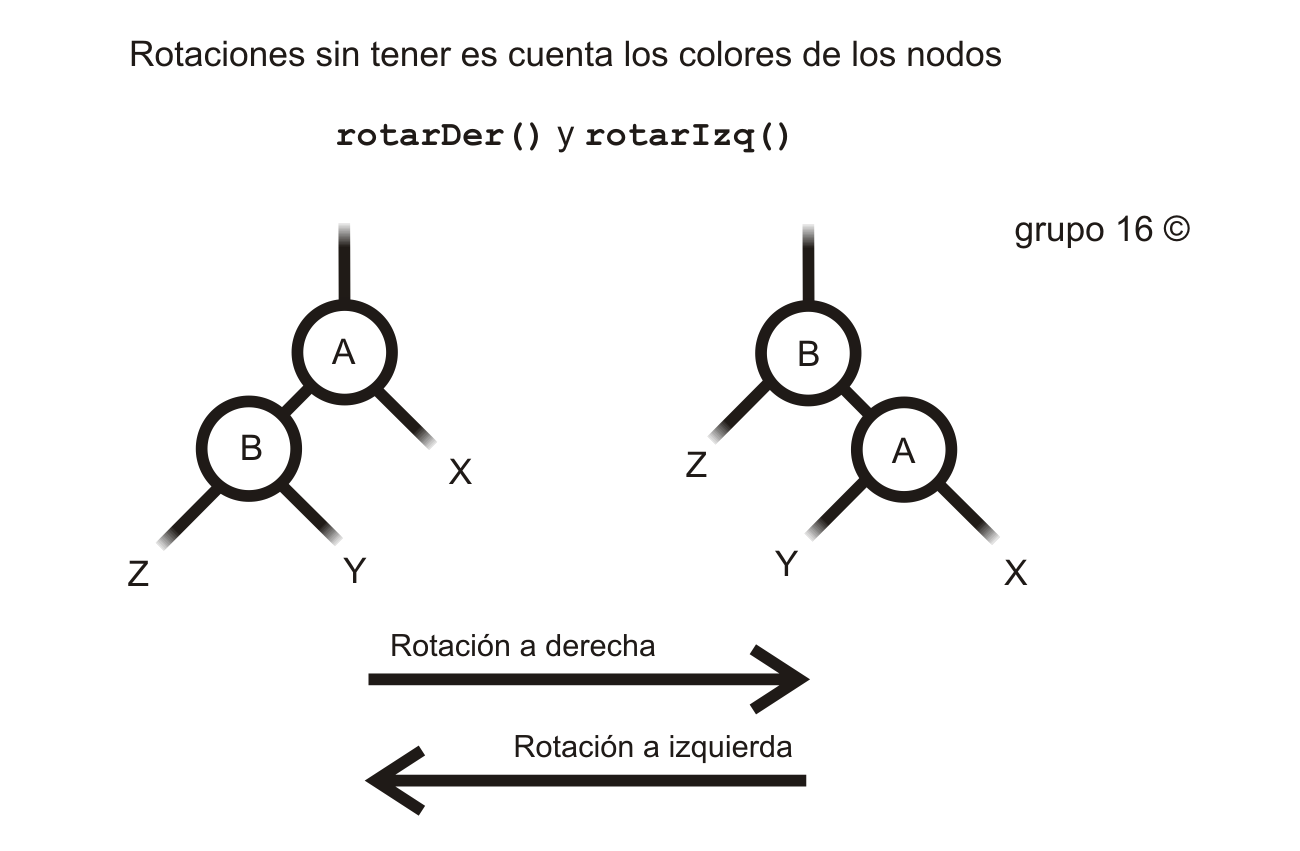
\includegraphics{rotaciones.png} \\
(figura 1.1)\\
\end{center}

Rotaciones simples para mantener el balanceo. (No son para hacerlo un AVL)

\subsection{CASO 1}

\begin{center}
		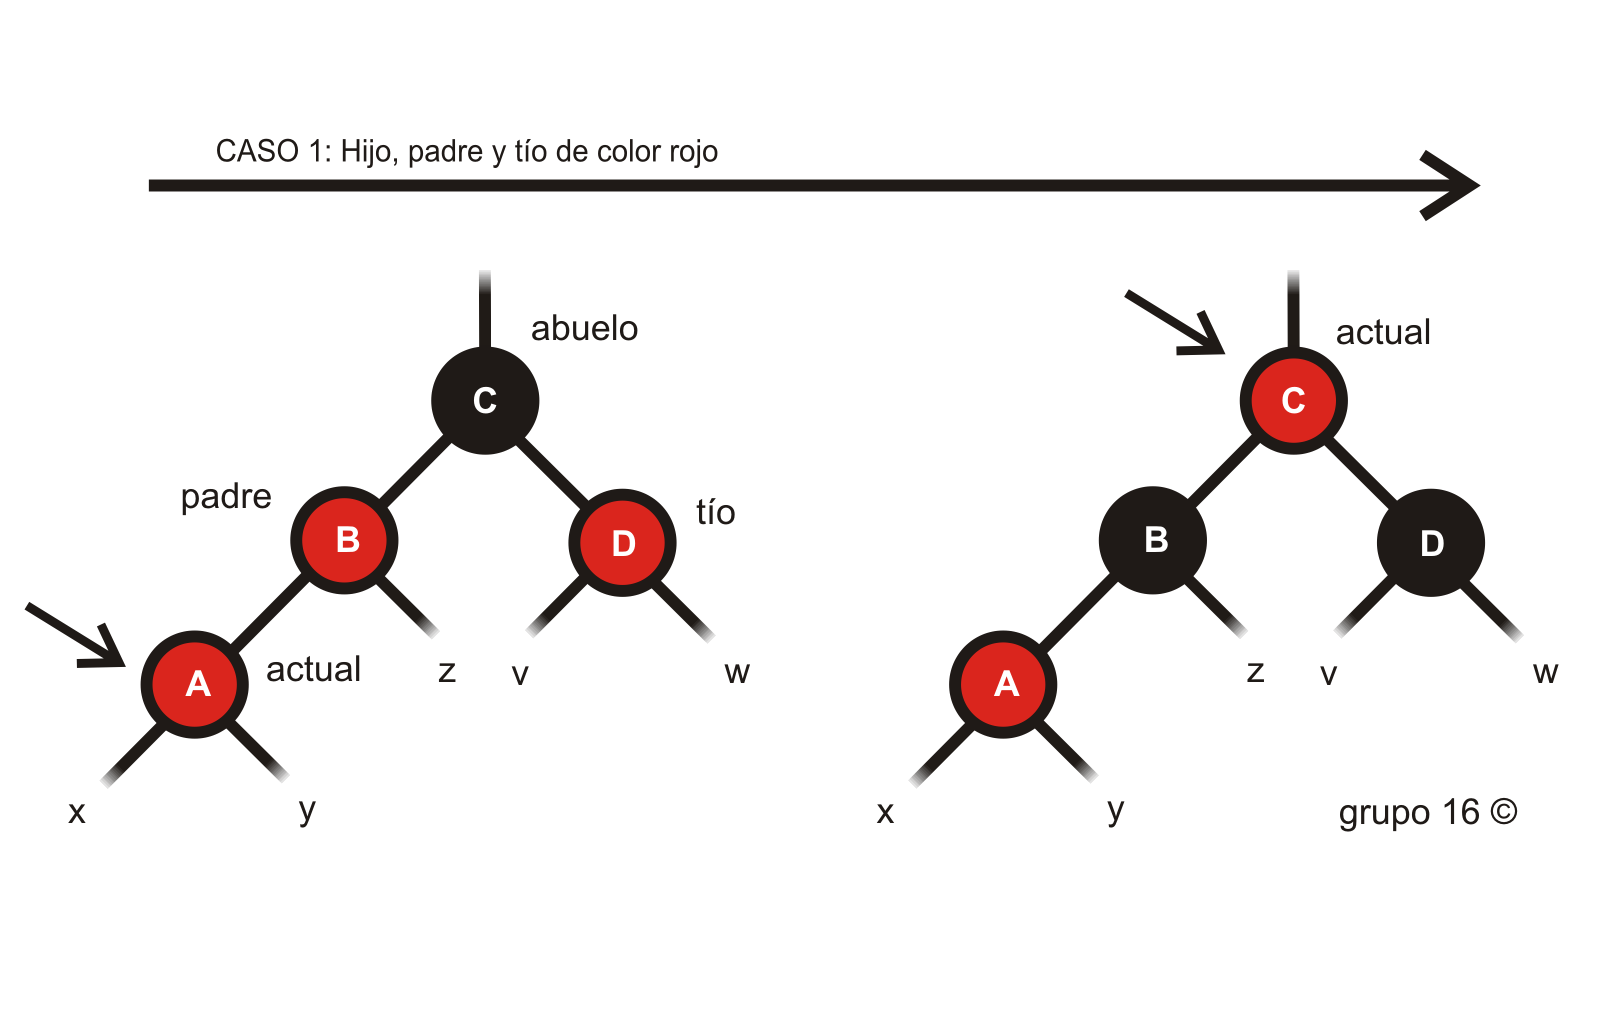
\includegraphics{caso1.png} \\
(figura 1.2)\\
\end{center}

Si A (Actual), B (Padre) y D (tio) son Rojos, estamos en \textsc{CASO 1}.\\
Pintamos al padre y tio de Negro, y pintamos a C (Abuelo) de Rojo. Como el arbol era un \rbt ese abuelo era negro.\\
Al hacer los cambios, alturas negras no se modifican. Por lo que hasta el abuelo tenemos todo arreglado.

\subsection{CASO 2}

\begin{center}
		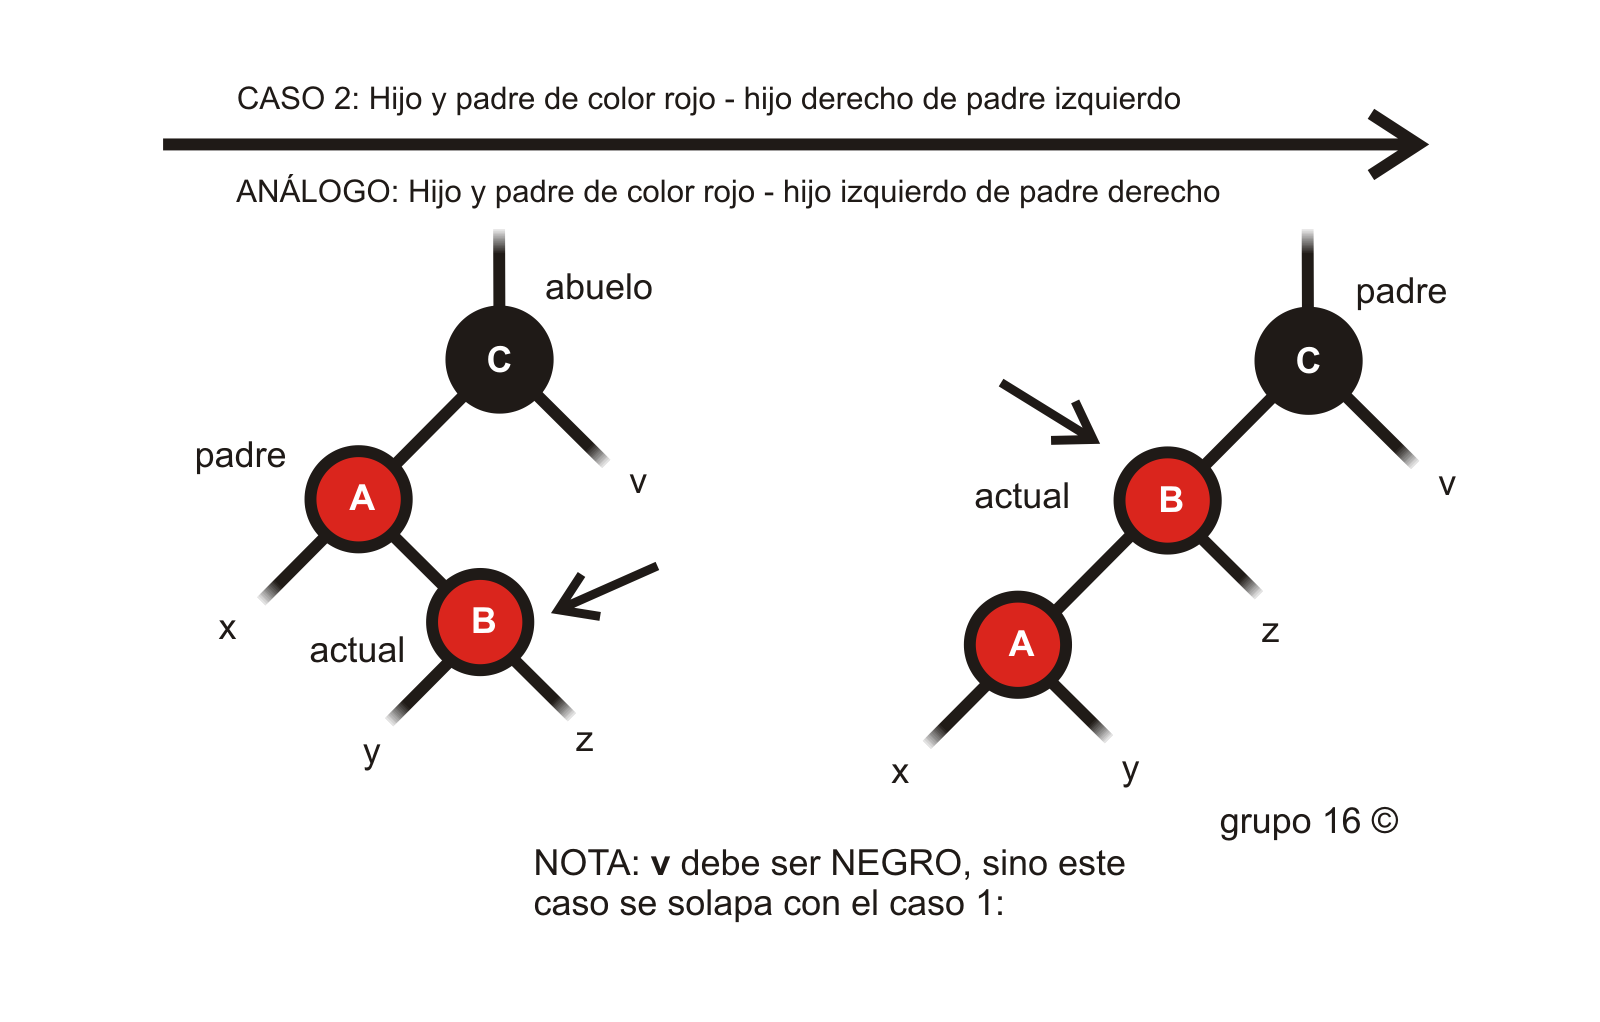
\includegraphics{caso2.png} \\
(figura 1.3)\\
\end{center}

Si B (Actual) y A (padre) son rojos y el tio es negro (o es nil - tambien considerado como regro) y ademas B es hijo derecho de un padre que es hijo izquierdo (o B es hijo izquierdo de un padre que es hijo derecho), estamos en \textsc{CASO 2}\\
Rotamos el padre a izquierda (o derecha segun el caso), y hemos reducido el \textsc{CASO 2} o un \textsc{CASO 3}.

\subsection{CASO 3}

\begin{center}
		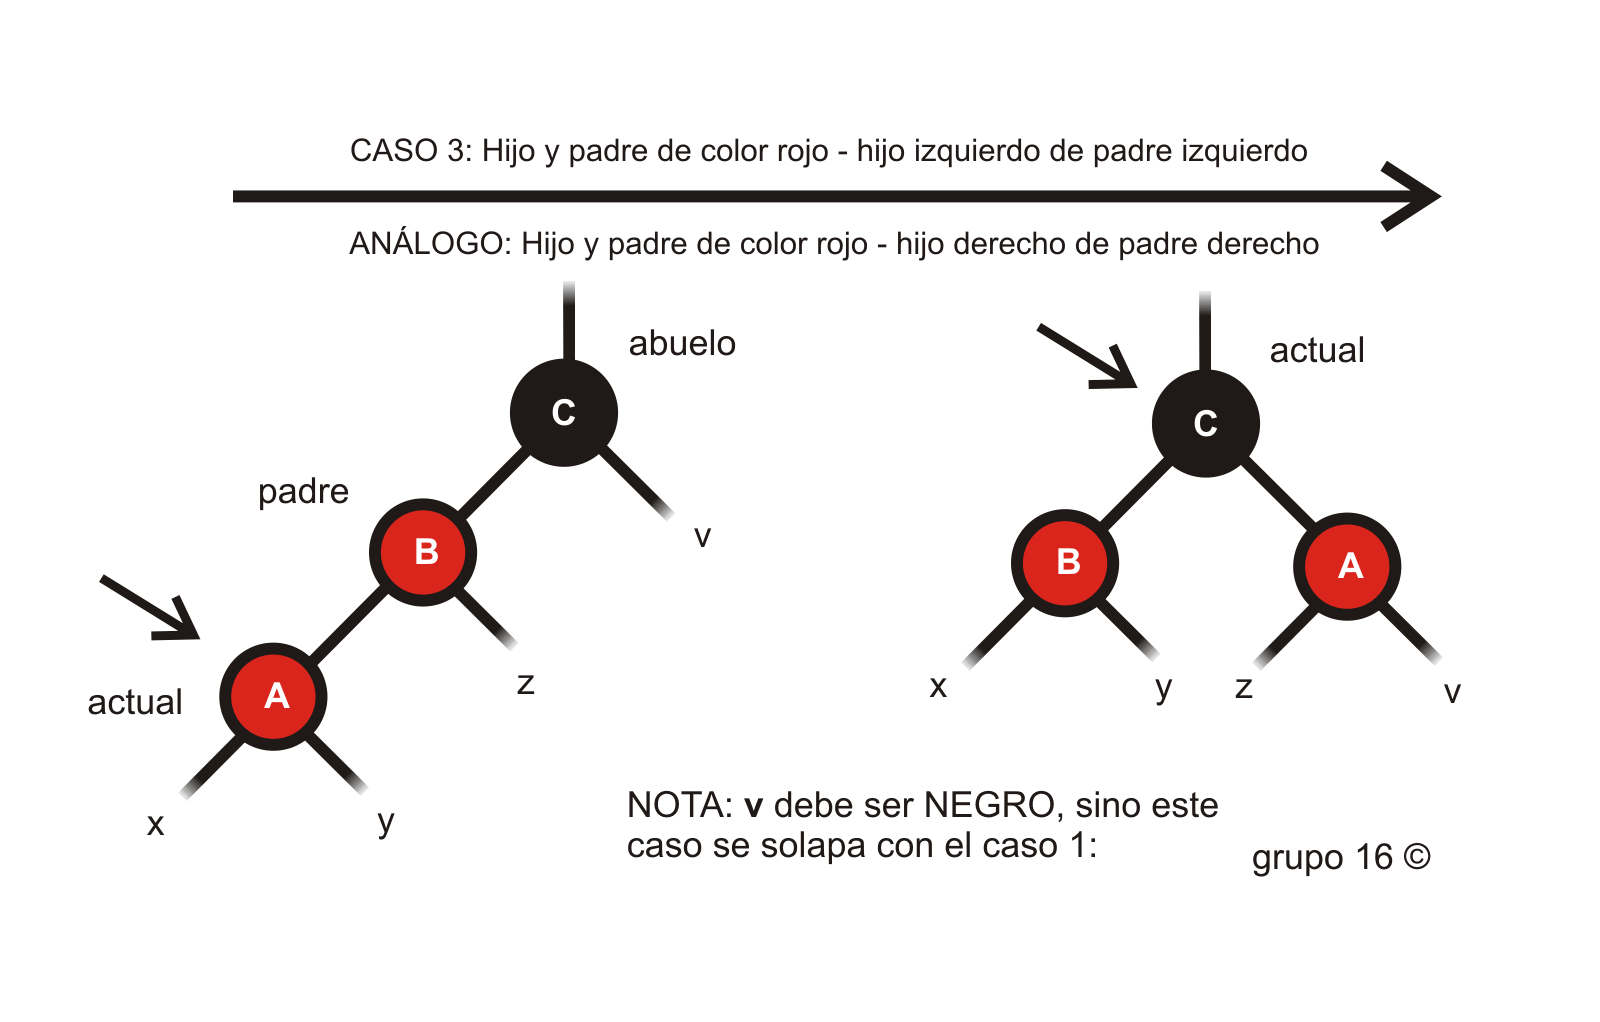
\includegraphics{caso3.png} \\
(figura 1.4)\\
\end{center}

Si A (Actual) y B (padre) son rojos y el tio es negro (o es nil - tambien considerado como regro) y ademas B es hijo derecho de un padre que es hijo derecho (o B es hijo izquierdo de un padre que es hijo izquierdo), estamos en \textsc{CASO 3}\\
Pintamos a padre negro, al abuelo rojo y y rotamos a derecha (o Izquerda segun el caso) al abuelo\\
Las alturas negras no se modifican y la posici�n del abuelo quedar�a negra, con ambos hijos rojo.

\subsection{TEST de Inserciones}

Hemos realizado un par de test para ``verificar'' el correcto fuincionemiento de las inserciones en el \rbt\\
Las inserciones fueron las siguientes $[10, 20, 15, 30, 40]$.\\
De esta manera probamos los casos mas interesantes:

\vskip0.3cm

\begin{tabular}{lll}
de $ninguno$ &			 a $[10]$ 					&	(CASO 0: Insertar raiz)\\
de $[10]$ &				 a $[10, 20]$				&	(CASO 0: Insertar con padres negro)\\
de $[10, 20]$ &			 a $[10, 20, 15]$ 			&	(CASO 2)\\
de $[10, 20, 15]$ &		 a $[10, 20, 15, 30]$ 		&	(CASO 1)\\
de $[10, 20, 15, 30]$ &	 a $[10, 20, 15, 30, 40]$ 	&	(CASO 3)\\
\end{tabular}
                                                                            
\vskip0.3cm

N�tese que en algunas de estas inserciones, \\
los llamados recursivos, llaman tambien a otros casos de ``reacomodacion''.\\
Para correr el test y observar la salida del programa se debe llamar al \verb|main| con parametro \verb|test|

\begin{center}
		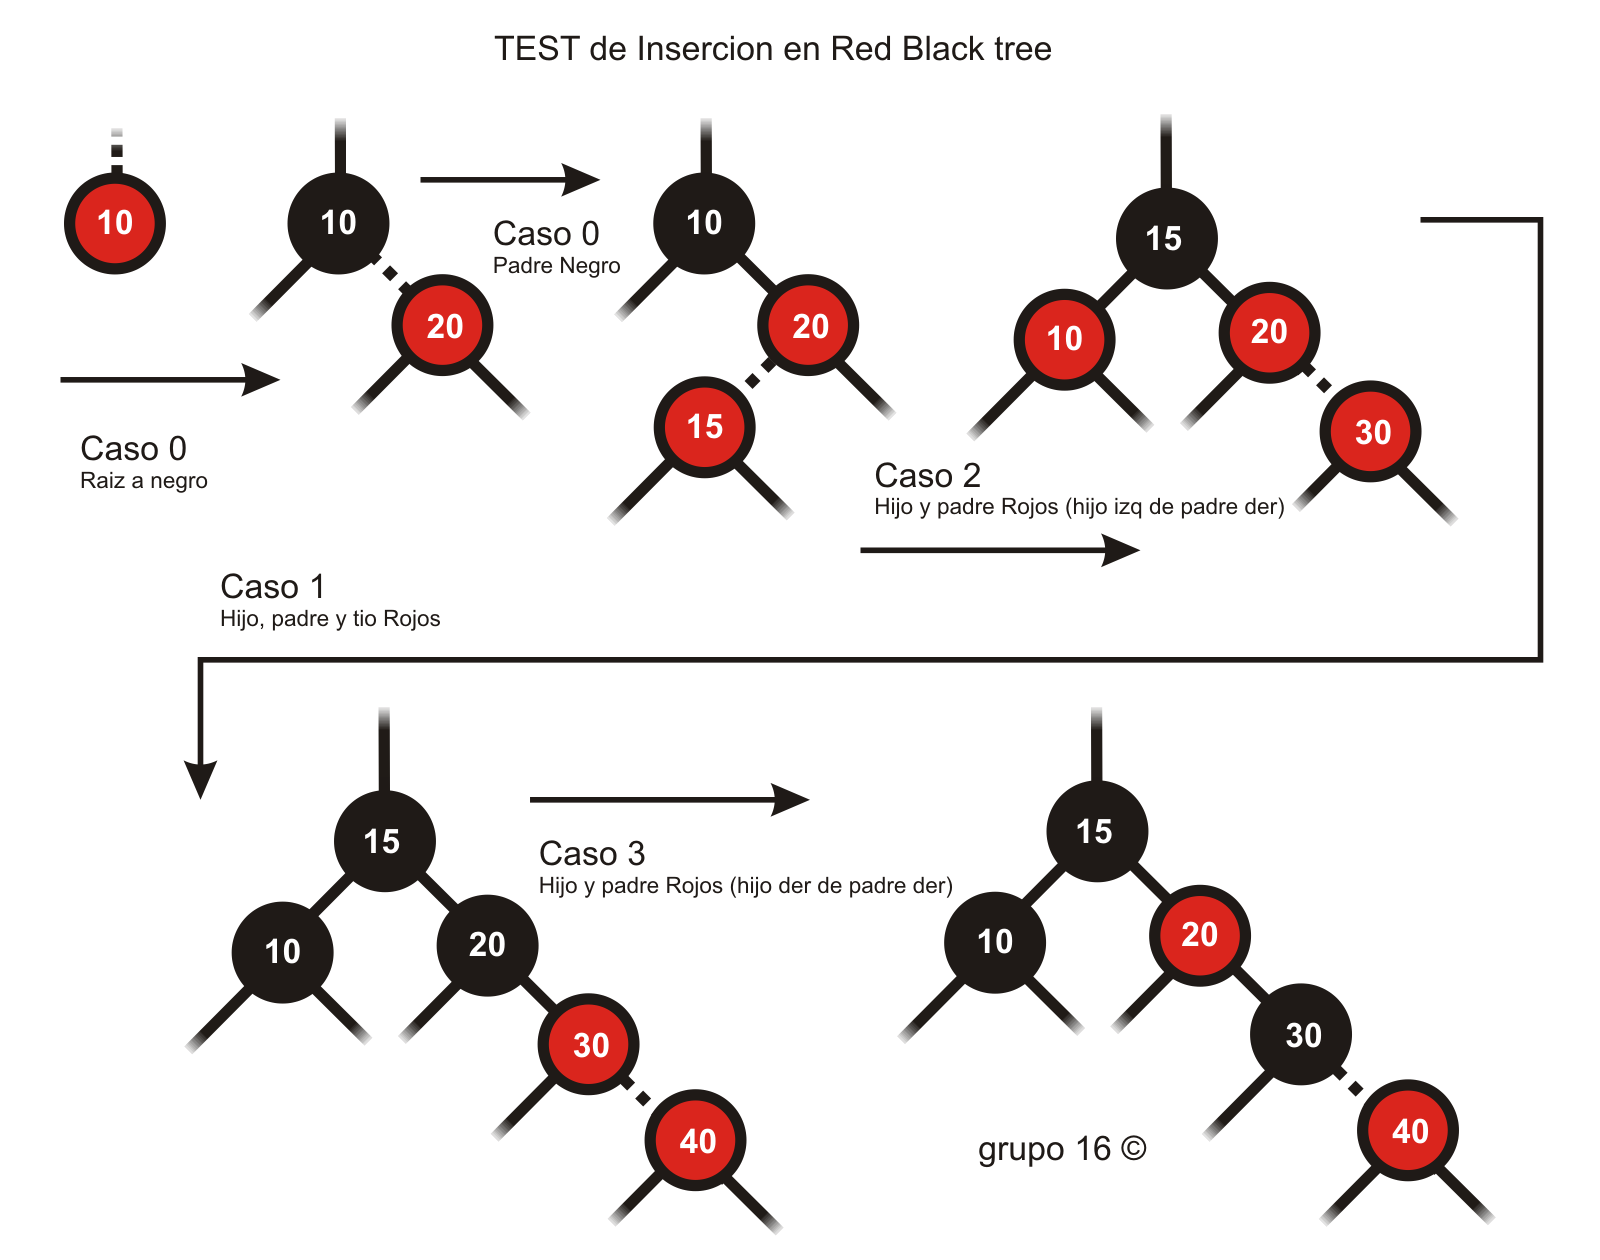
\includegraphics{test_insercion.png} \\
(figura 1.5)\\
\end{center}

\vskip0.5cm

\section{\adi}

\subsection{Ideas para la eleccion de estructura del \adi}

%//////////////////////////////////////////////////////////////////

\subsubsection{Dos �rboles}

La primera idea que se nos acurrio para extender el arbol de intervalos a dos dimenciones, fue simplemente tener dos �rboles (uno para cada coordenada).\\
La busqueda entonces consistia en buscar las imagenes correspondientes al la coordenada $x$ y luego las imagenes correspondientes a la coordenada $y$. Por ultimo, debiamos encontrar las imagenes que aparecieran en los dos conjuntos.

\vskip0.3cm

\Large Costo temporal de la construccion \normalsize

\vskip0.3cm

\Large Costo espacial de la construccion \normalsize

\vskip0.3cm

\Large Costo temporal total de la consulta \normalsize

\vskip0.3cm

\Large Costo espacial de la consulta  \normalsize

%//////////////////////////////////////////////////////////////////

\subsubsection{�rbol con ambas coordenadas}

Otra idea fue, hacer un solo arbol en el que los ``Intervalos Elementales'' se construyeran con todos los puntos de inicio y finalizacion de las coordenadas $x$ e $y$. En cada nodo de este arbol se encontrabas un arreglo (o alguna otra estructura) con las imagenes que le correspondian en $x$ y otro arreglo con las imagenes que le correspondian en $y$.\\
De esta manera teniamos un solo arbol y espacialmente reduciamos la cantidad de nodos existentes. (La cantidad de nodos con dos arboles era 

	\[\#\{IntervalosElementales(x)\} + \{IntervalosElementales(y)\}\]
	
y de esta manera era 

	\[\#(\{IntervalosElementales(x)\} \cup \{IntervalosElementales(y)\})\]

\vskip0.3cm

\Large Costo temporal de la construccion \normalsize

\vskip0.3cm

\Large Costo espacial de la construccion \normalsize

\vskip0.3cm

\Large Costo temporal total de la consulta \normalsize

\vskip0.3cm

\Large Costo espacial de la consulta \normalsize

%//////////////////////////////////////////////////////////////////

\subsubsection{�rboles dentro de �rbol}

...

\vskip0.3cm

\Large Costo temporal de la construccion \normalsize

\vskip0.3cm

\Large Costo espacial de la construccion \normalsize

\vskip0.3cm

\Large Costo temporal total de la consulta \normalsize

\vskip0.3cm

\Large Costo espacial de la consulta \normalsize


%//////////////////////////////////////////////////////////////////

\subsubsection{�rboles unico (en alguna de las dos coordenadas)}

...

\vskip0.3cm

\Large Costo temporal de la construccion \normalsize

\vskip0.3cm

\Large Costo espacial de la construccion \normalsize

\vskip0.3cm

\Large Costo temporal total de la consulta \normalsize

\vskip0.3cm

\Large Costo espacial de la consulta \normalsize

%//////////////////////////////////////////////////////////////////

\subsection{Conculciones sobre los algoritmos y eleccion}


\vskip0.5cm
%\newpage
%\section{Ejercicio 2}

%\subsection{insertar en \rbt}

%\subsection{insertar en \adi}


\begin{itemize}
\item \textit{prepararArregloEstanImagenes(int im)}

inicializa un arreglo en false\\
Costo $O(im)$

\item \textit{intervalosElementales(Lista(imagenes) img) $->$ Conj(puntos):res}

\begin{framed}
\begin{verbatimtab}[4]
intervalosElementales(Lista(imagenes) img) -> Conj(puntos):res
{
	desde 0 a Tam(img) hacer	// O(1) / itera im veces
	{
		res <- agregar(x_0)		// O(log(2im))
		res <- agregar(x_1)		// O(log(2im))
	}
	return res					// O(1)
}
\end{verbatimtab}
\end{framed}

Como ingresamos dos puntos por imagen a lo sumo el conjunto tendra $2im$, por lo que pudimos acotar la insercion $log(2im)$.\\
El costo total de este algoritmo es pues $O(im*log(im))$
            
\item \textit{insertar(IntervaloElemental ie)}

\item \textit{llenarIntervalosElementales(Lista(Imagen):imagenes, bool:X)}
\begin{framed}
\begin{verbatimtab}[4]          
llenarIntervalosElementales(Lista(Imagen):imagenes, bool:X)
{
	Conj(IntervaloElemental):puntos = intervalosElementales(imagenes, X);	
										// O(im*log(im))

	por cada imagen de "imagenes"		// itera im veces
		insertar(elemento)				// O(log(n))
}
\end{verbatimtab}
\end{framed}

Entonces la complejidad de insertar todos los intervalos elementales es\\
$O(im*log(im)) + O(im*log(n))$
            
\item \textit{insertarImagen(int indiceImagen, inicio, final, min, max, Nodo actual)}
      
\item \textit{insertarImagenes(Lista(Imagen):imagenes, bool:X)}
\begin{framed}
\begin{verbatimtab}[4]
insertarImagenes(Lista(Imagen):imagenes, bool:X)
{
	depeniendo de si es por X o por Y
		por cada imagnen de "imagenes"
			insertarImagen(i, inicio, fin, 0, ANCHO_ARBOL, raiz);
}
\end{verbatimtab}
\end{framed}

\item \textit{llenarArbol( Lista(Imagen):imagenes, bool:X) $->$ ArbolDeIntervalos}
\begin{framed}
\begin{verbatimtab}[4]          
llenarArbol( Lista(Imagen):imagenes, bool:X) -> ArbolDeIntervalos
{
	prepararArregloEstanImagenes(im);
	llenarIntervalosElementales(imagenes, X);
	insertarImagenes(imagenes, X);
}
\end{verbatimtab}
\end{framed}




\end{itemize}	

 
            
\begin{itemize}

\item \textit{buscarIndices(int punto, Nodo actual, conj(int))}
\begin{framed}
\begin{verbatimtab}[4]
buscarIndices(int punto, Nodo actual, conj(int))
{
	si no llegue al final del arbol
		res <- agregar(los indices que aparecen en el nodo)
		{
		si  punto es <= actual_numero
			buscarIndices(punto, Izq(actual), conj(int))
		si  punto es >= actual_numero
			buscarIndices(punto, Der(actual), conj(int))		
		}
}
\end{verbatimtab}
\end{framed}

Este es un algoritmo recursivo, que separa siempre el problema es dos partes iguales.\\
�Entra siempre por las dos ramas?... No\\
Existe a lo sumo solo un nodo en el arbol que tiene el mismo valor que el punto buscado, por lo tanto el algoritmo, hace a lo sumo dos caminos.\\
Que recorra uno o dos caminos es despreciable, por lo que su complejidad se puede expresar de la siguinte manera.
\[
\left\{
\displaystyle\matrix{
T(0) = d\hfill\cr
T(n) = T(n/2) + c + k_i
} 
\right.
\]
desarrollando una vez 
\[T(n) = T(n/4) + c + k_i + c + k_j\]
la formula general es
\[T(n) = T(n/2^h) + h*c + \displaystyle\sum_{i=1}^h k_i \]
con $h$ es la altura del arbol\\
como es un \rbt la altura es cercana a $log(n)$
\[T(n) = T(n/2^{log(n)}) + log(n)*c + \displaystyle\sum_{i=1}^h k_i\]
como a cada imagen la incuentro una sola vez por camino (pues si la encontre en un nodo no puedo escontrarla en sus hijos), habr� encontrado al final mis $k$ imagenes buscadas.
\[T(n) = T(n/n) + log(n)*c + k\]
\[T(n) = T(1) + log(n)*c + k\]
Esto da un complejidad total de $O(log(n) + k)$.

\item \textit{busqueda(x, y, Lista(Imagen):Imagenes\_levantadas, bool:X) $->$ Lista(Imagen)}
\begin{framed}
\begin{verbatimtab}[4]
busqueda(x, y, Lista(Imagen):Imagenes_levantadas, bool:X) -> Lista(Imagen):res
{
	dependiendo si es por X o por Y					// O(1)
		Lista(int):resIndices;						// O(1)
		buscarIndices(x, raiz, resIndices);			// O(log(n) + k)

		desde i=0 a Tam(resIndices) hacer			// itera k veces
		{			
			si esta entre los valores de y o x		// O(1)
				agregar imagen al resutado			// O(1)
			borrar del vector EstanImagenes			// O(1)
		}		
}
\end{verbatimtab}
\end{framed}

Este algoritmo es simple, consigue los indices de las imagenes que debe agregar segun una de las coordendas ($x$ o $y$) y vesifica luego que cumpla la otra coordenada tambien

Complejidad: $O(2 + log(n) + k + 3k) = O(log(n) + k)$

\end{itemize}



%\[
%T(n) = 
%\left\{
%\displaystyle\matrix{
%d & n=0\cr
%T(n/2) + c + k_i & n>0
%} 
%\right.
%\]
%\displaystyle\sum_{k=1}^N k^2 
% ${x+1 \brace x-1}$
%$\displaystyle\matrix{\strut\hbox{1}\hfill\cr\strut\hbox{2}\hfill\cr}$
%\newpage
%\tableofcontents
	
\end{document}

